\section{Supervised Optimization Operator Evaluation}
In our main experiment, we compare the effectivity of 4 optimization operators on 3 diverse gold-labeled datasets.
We will compare the results and costs of each method against each other and a strong Instruction Induction baseline.

All our experiments were conducted throught the \texttt{OpenRouter API}, which offers many LLMs from different providers.
We will differentiate between optimizer LLM $\mathcal(M)_{\text{optim}}$ and $\mathcal(M)_{\text{solve}}$.
Both use the medium model \texttt{Google Gemma 3 27B}\cite{gemmateam2025gemma3technicalreport}. 
To encourage diversity, $\mathcal(M)_{\text{optim}}$ works with sampling temperature $\tau = 0.75$. 
Bigger sampling temperature was observed to diminish the model's ability to follow structured output specifications.
To keep prompt testing as deterministic as possible, we initialize $\mathcal(M)_{\text{solve}}$ with $\tau = 0.0$.


\subsection{Experiment setup}
We test our method against 3 datasets, \texttt{CodeContests}, \texttt{Connections}  and \texttt{Sequences}, which have 30 samples each 
and form 3 equal splits $\mathcal{D}_{\text{train}}$, $\mathcal{D}_{\text{dev}}$ and $\mathcal{D}_{\text{test}}$. Each out of the 4 operators - \texttt{Reflective}, \texttt{Iterative}, \texttt{Feedback} and \texttt{Paraphrase} - is tested on all three datasets for 3 repetitions
to alleviate randomness in the results.

To create a strong baseline, we begin by creating $50$ prompts $\mathcal{P}_{\text{baseline}}$ with Instruction Induction through the \texttt{Lamarckian} operator 
using \texttt{Persona}\cite{ge2024scalingsyntheticdatacreation} seeding. These prompts form $\mathcal{P}_{\text{baseline}}$. Examples are sampled from $\mathcal{D}_{\text{train}}$ with the whole 10 sample split being used for \texttt{Connections} and \texttt{Sequences}
and 3 samples for \texttt{CodeContests}. This is because code input/output pairs are a lot longer and we observed a greater likelihood of failure to follow output structure for more samples.

These $50$ prompts are evaluated on $\mathcal{D}_{\text{test}}$ and the second quintile (prompts 11-20 when ranked by test score) is used as the initial population $\mathcal{P}_{\text{init}}$ for the optimizer.
We use population size $S=10$, iteration count $I=10$, batch size $B=3$ and pruning factor $f_{\text{prune}} = 0.5$. This means that each step produces $5$ new prompts and $50$ prompts overall.
We select these parameters to make the optimization process resources \textit{roughly} comparable to the Instruction Induction baseline generation.


\subsection{Experiment results}
In tables \ref{tab:rescodecontests}, \ref{tab:resconnections} and \ref{tab:ressequences} we results of our 
main experiment on \texttt{CodeContests}, \texttt{Connections} and \texttt{Sequences} respectively.
In the row \textit{Baseline}, we present the maximum score achieved by prompts $P\in\mathcal{P}_{\text{baseline}}$. 
This forms the hard baseline. The next row, \textit{Initial}, shows the best score out of the initializing prompts $P\in\mathcal{P}_{\text{init}}$.
The following rows show the average of each optimization step's $s$ maximum score over all three experiment repetitions $e\in\{1,2,3\}$:
\begin{equation}
    \frac{1}{3}\sum_{e=1}^{3}\operatorname{Max}(\mathcal{E}_{\mathcal{D}_{\text{test}}}(\mathcal{P}_{s}^{e})),
\end{equation}
where $\mathcal{P}_{s}^{e}$ signifies the population at step $s$ of experiment repetition $e$.
For each operator, the best step score is marked in \textbf{bold} and the best score overall is also \underline{underlined}.
We also include the average score in  bracketed smaller script, defined by 
\begin{equation}
    \frac{1}{3}\sum_{e=1}^{3}\operatorname{Mean}(\mathcal{E}_{\mathcal{D}_{\text{test}}}(\mathcal{P}_{s}^{e})).
\end{equation}

\begin{table}[htbp]
    \centering
    \captionsetup{font=small}
    \caption{Results for codecontests}  
    \label{tab:rescodecontests}
    \renewcommand{\arraystretch}{1.4} % row spacing

    \begin{tabular}{|c||c|c|c|c|}
    \hline
    \rowcolor{ctulightblue}
    \textsc{Step} &
    \cellcolor{ctulightblue}\textsc{Reflective} &
    \cellcolor{ctulightblue}\textsc{Iterative} &
    \cellcolor{ctulightblue}\textsc{Feedback} &
    \cellcolor{ctulightblue}\textsc{Paraphrase} \\
    \hline

    \rowcolor{ctuorange!15}
    Baseline & 0.26 & 0.26 & 0.26 & 0.26 \\ \hline
Initial & 0.16 & 0.16 & 0.16 & 0.16 \\ \hline
$1$ & \cellcolor{lightgreen}\maxmean{0.23}{0.15} & \cellcolor{lightgreen}\maxmean{0.17}{0.12} & \cellcolor{lightgreen}\maxmean{0.26}{0.15} & \cellcolor{lightgreen}\maxmean{0.22}{0.14} \\ \hline
$2$ & \cellcolor{lightgreen}\maxmean{0.22}{0.12} & \cellcolor{lightgreen}\maxmean{0.25}{0.16} & \cellcolor{lightred}\maxmean{0.11}{0.06} & \cellcolor{lightgreen}\maxmean{0.22}{0.14} \\ \hline
$3$ & \cellcolor{lightgreen}\maxmean{0.23}{0.15} & \cellcolor{lightgreen}\maxmean{0.19}{0.12} & \cellcolor{lightred}\maxmean{0.16}{0.07} & \cellcolor{lightgreen}\maxmean{0.19}{0.14} \\ \hline
$4$ & \cellcolor{lightgreen}\maxmean{0.18}{0.14} & \cellcolor{lightgreen}\maxmean{0.27}{0.15} & \cellcolor{lightred}\maxmean{0.09}{0.05} & \cellcolor{lightgreen}\maxmean{0.19}{0.14} \\ \hline
$5$ & \cellcolor{lightgreen}\maxmean{0.23}{0.17} & \cellcolor{lightred}\maxmean{0.16}{0.11} & \cellcolor{lightred}\maxmean{0.09}{0.05} & \cellcolor{lightgreen}\maxmean{0.22}{0.14} \\ \hline
$6$ & \cellcolor{lightgreen}\maxmean{0.23}{0.17} & \cellcolor{lightgreen}\maxmean{0.18}{0.11} & \cellcolor{lightred}\maxmean{0.08}{0.04} & \cellcolor{lightgreen}\maxmean{0.23}{0.14} \\ \hline
$7$ & \cellcolor{lightgreen}\maxmean{0.25}{0.16} & \cellcolor{lightgreen}\maxmean{0.25}{0.13} & \cellcolor{lightred}\maxmean{0.05}{0.04} & \cellcolor{lightgreen}\maxmean{0.19}{0.12} \\ \hline
$8$ & \cellcolor{lightred}\maxmean{0.15}{0.12} & \cellcolor{lightgreen}\maxmean{0.23}{0.16} & \cellcolor{lightred}\maxmean{0.08}{0.05} & \cellcolor{lightgreen}\maxmean{0.17}{0.11} \\ \hline
$9$ & \cellcolor{lightgreen}\maxmean{0.23}{0.14} & \cellcolor{lightgreen}\maxmean{0.19}{0.11} & \cellcolor{lightred}\maxmean{0.15}{0.07} & \cellcolor{lightgreen}\maxmean{0.17}{0.12} \\ \hline
$10$ & \cellcolor{lightgreen}\maxmean{0.24}{0.13} & \cellcolor{lightgreen}\maxmean{0.25}{0.13} & \cellcolor{lightred}\maxmean{0.08}{0.04} & \cellcolor{lightgreen}\maxmean{0.23}{0.15} \\ \hline


    \end{tabular}
\end{table}

\begin{table}[htbp]
    \centering
    \captionsetup{font=small}
    \caption{Results for connections}  
    \label{tab:resconnections}
    \renewcommand{\arraystretch}{1.4} % row spacing

    \begin{tabular}{|c||c|c|c|c|}
    \hline
    \rowcolor{ctulightblue}
    \textsc{Step} &
    \cellcolor{ctulightblue}\textsc{Reflective} &
    \cellcolor{ctulightblue}\textsc{Iterative} &
    \cellcolor{ctulightblue}\textsc{Feedback} &
    \cellcolor{ctulightblue}\textsc{Paraphrase} \\
    \hline

    \rowcolor{ctuorange!15}
    Baseline & 0.33 & 0.33 & 0.33 & 0.33 \\ \hline
Initial & 0.20 & 0.20 & 0.20 & 0.20 \\ \hline
$1$ & \cellcolor{lightgreen}\maxmean{0.29}{0.15} & \cellcolor{lightgreen}\maxmean{0.27}{0.16} & \cellcolor{lightgreen}\maxmean{0.20}{0.15} & \cellcolor{lightgreen}\maxmean{0.31}{0.21} \\ \hline
$2$ & \cellcolor{lightgreen}\maxmean{0.20}{0.13} & \cellcolor{lightgreen}\maxmean{0.29}{0.18} & \cellcolor{lightgreen}\maxmean{0.24}{0.14} & \cellcolor{lightgreen}\maxmean{0.32}{0.20} \\ \hline
$3$ & \cellcolor{lightgreen}\maxmean{0.20}{0.14} & \cellcolor{lightgreen}\maxmean{0.27}{0.17} & \cellcolor{lightred}\maxmean{0.19}{0.14} & \cellcolor{lightgreen}\maxmean{0.29}{0.21} \\ \hline
$4$ & \cellcolor{lightred}\maxmean{0.18}{0.04} & \cellcolor{lightgreen}\maxmean{0.26}{0.17} & \cellcolor{lightred}\maxmean{0.09}{0.06} & \cellcolor{lightgreen}\maxmean{0.28}{0.19} \\ \hline
$5$ & \cellcolor{lightred}\maxmean{0.16}{0.08} & \cellcolor{lightgreen}\maxmean{0.27}{0.18} & \cellcolor{lightred}\maxmean{0.14}{0.09} & \cellcolor{lightgreen}\maxmean{0.31}{0.20} \\ \hline
$6$ & \cellcolor{lightred}\maxmean{0.17}{0.09} & \cellcolor{lightgreen}\maxmean{0.27}{0.19} & \cellcolor{lightred}\maxmean{0.13}{0.08} & \cellcolor{lightgreen}\maxmean{0.32}{0.21} \\ \hline
$7$ & \cellcolor{lightred}\maxmean{0.16}{0.08} & \cellcolor{lightgreen}\maxmean{0.29}{0.19} & \cellcolor{lightred}\maxmean{0.10}{0.04} & \cellcolor{lightgreen}\maxmean{0.30}{0.19} \\ \hline
$8$ & \cellcolor{lightred}\maxmean{0.16}{0.08} & \cellcolor{lightgreen}\maxmean{0.28}{0.19} & \cellcolor{lightred}\maxmean{0.07}{0.04} & \cellcolor{lightgreen}\maxmean{0.33}{0.23} \\ \hline
$9$ & \cellcolor{lightred}\maxmean{0.16}{0.07} & \cellcolor{lightgreen}\maxmean{0.27}{0.20} & \cellcolor{lightred}\maxmean{0.05}{0.03} & \cellcolor{lightgreen}\maxmean{0.28}{0.22} \\ \hline
$10$ & \cellcolor{lightred}\maxmean{0.16}{0.07} & \cellcolor{lightgreen}\maxmean{0.26}{0.16} & \cellcolor{lightred}\maxmean{0.07}{0.03} & \cellcolor{lightgreen}\maxmean{0.35}{0.25} \\ \hline


    \end{tabular}
\end{table}

\begin{table}[htbp]
    \centering
    \captionsetup{font=small}
    \caption{Results for sequences}  
    \label{tab:ressequences}
    \renewcommand{\arraystretch}{1.4} % row spacing

    \begin{tabular}{|c||c|c|c|c|}
    \hline
    \rowcolor{ctulightblue}
    \textsc{Step} &
    \cellcolor{ctulightblue}\textsc{Reflective} &
    \cellcolor{ctulightblue}\textsc{Iterative} &
    \cellcolor{ctulightblue}\textsc{Feedback} &
    \cellcolor{ctulightblue}\textsc{Paraphrase} \\
    \hline

    \rowcolor{ctuorange!15}
    Baseline & 0.70 & 0.70 & 0.70 & 0.70 \\ \hline
Initial & 0.40 & 0.40 & 0.40 & 0.40 \\ \hline
$1$ & \cellcolor{lightgreen}\maxmean{0.47}{0.23} & \cellcolor{lightgreen}\maxmean{0.63}{0.36} & \cellcolor{lightgreen}\maxmean{0.43}{0.29} & \cellcolor{lightgreen}\maxmean{0.73}{0.38} \\ \hline
$2$ & \cellcolor{lightgreen}\maxmean{0.53}{0.39} & \cellcolor{lightgreen}\maxmean{0.53}{0.32} & \cellcolor{lightgreen}\maxmean{0.47}{0.32} & \cellcolor{lightgreen}\maxmean{0.60}{0.33} \\ \hline
$3$ & \cellcolor{lightred}\maxmean{0.27}{0.15} & \cellcolor{lightgreen}\maxmean{0.67}{0.43} & \cellcolor{lightgreen}\maxmean{0.47}{0.33} & \cellcolor{lightgreen}\maxmean{0.63}{0.37} \\ \hline
$4$ & \cellcolor{lightgreen}\maxmean{0.47}{0.21} & \cellcolor{lightgreen}\maxmean{0.63}{0.42} & \cellcolor{lightgreen}\maxmean{0.47}{0.32} & \cellcolor{lightgreen}\maxmean{0.60}{0.42} \\ \hline
$5$ & \cellcolor{lightgreen}\maxmean{0.57}{0.33} & \cellcolor{lightgreen}\maxmean{0.63}{0.40} & \cellcolor{lightred}\maxmean{0.40}{0.28} & \cellcolor{lightgreen}\maxmean{0.60}{0.38} \\ \hline
$6$ & \cellcolor{lightgreen}\maxmean{0.53}{0.35} & \cellcolor{lightgreen}\maxmean{0.57}{0.34} & \cellcolor{lightred}\maxmean{0.27}{0.19} & \cellcolor{lightgreen}\maxmean{0.80}{0.45} \\ \hline
$7$ & \cellcolor{lightgreen}\maxmean{0.57}{0.44} & \cellcolor{lightgreen}\maxmean{0.60}{0.31} & \cellcolor{lightred}\maxmean{0.37}{0.23} & \cellcolor{lightgreen}\maxmean{0.73}{0.37} \\ \hline
$8$ & \cellcolor{lightgreen}\maxmean{0.63}{0.46} & \cellcolor{lightgreen}\maxmean{0.70}{0.50} & \cellcolor{lightred}\maxmean{0.37}{0.25} & \cellcolor{lightgreen}\maxmean{0.57}{0.29} \\ \hline
$9$ & \cellcolor{lightgreen}\maxmean{0.50}{0.40} & \cellcolor{lightgreen}\maxmean{0.80}{0.37} & \cellcolor{lightgreen}\maxmean{0.43}{0.27} & \cellcolor{lightgreen}\maxmean{0.63}{0.44} \\ \hline
$10$ & \cellcolor{lightgreen}\maxmean{0.57}{0.41} & \cellcolor{lightgreen}\maxmean{0.57}{0.39} & \cellcolor{lightred}\maxmean{0.33}{0.21} & \cellcolor{lightgreen}\maxmean{0.60}{0.35} \\ \hline


    \end{tabular}
\end{table}



\begin{table}[htbp]
    \centering
    \captionsetup{font=small}
    \caption{Results for codecontests}  
    \label{tab:rescodecontests}
    \renewcommand{\arraystretch}{1.4} % row spacing

    \begin{tabular}{|c||c|c|c|c|}
    \hline
    \rowcolor{ctulightblue}
    \textsc{Step} &
    \cellcolor{ctulightblue}\textsc{Reflective} &
    \cellcolor{ctulightblue}\textsc{Iterative} &
    \cellcolor{ctulightblue}\textsc{Feedback} &
    \cellcolor{ctulightblue}\textsc{Paraphrase} \\
    \hline

    \rowcolor{ctuorange!15}
    Baseline & \textbf{0.26} & 0.26 & \textbf{0.26} & \textbf{0.26} \\ \hline
Initial & 0.16 & 0.16 & 0.16 & 0.16 \\ \hline
$1$ & \maxmean{0.23}{0.15} & \maxmean{0.17}{0.12} & \maxmean{\textbf{0.26}}{0.15} & \maxmean{0.22}{0.14} \\ \hline
$2$ & \maxmean{0.22}{0.12} & \maxmean{0.25}{0.16} & \maxmean{0.11}{0.06} & \maxmean{0.22}{0.14} \\ \hline
$3$ & \maxmean{0.23}{0.15} & \maxmean{0.19}{0.12} & \maxmean{0.16}{0.07} & \maxmean{0.19}{0.14} \\ \hline
$4$ & \maxmean{0.18}{0.14} & \maxmean{\underline{\textbf{0.27}}}{0.15} & \maxmean{0.09}{0.05} & \maxmean{0.19}{0.14} \\ \hline
$5$ & \maxmean{0.23}{0.17} & \maxmean{0.16}{0.11} & \maxmean{0.09}{0.05} & \maxmean{0.22}{0.14} \\ \hline
$6$ & \maxmean{0.23}{0.17} & \maxmean{0.18}{0.11} & \maxmean{0.08}{0.04} & \maxmean{0.23}{0.14} \\ \hline
$7$ & \maxmean{0.25}{0.16} & \maxmean{0.25}{0.13} & \maxmean{0.05}{0.04} & \maxmean{0.19}{0.12} \\ \hline
$8$ & \maxmean{0.15}{0.12} & \maxmean{0.23}{0.16} & \maxmean{0.08}{0.05} & \maxmean{0.17}{0.11} \\ \hline
$9$ & \maxmean{0.23}{0.14} & \maxmean{0.19}{0.11} & \maxmean{0.15}{0.07} & \maxmean{0.17}{0.12} \\ \hline
$10$ & \maxmean{0.24}{0.13} & \maxmean{0.25}{0.13} & \maxmean{0.08}{0.04} & \maxmean{0.23}{0.15} \\ \hline
    \end{tabular}
\end{table}

\begin{figure}
    \label{fig:codecontests}
    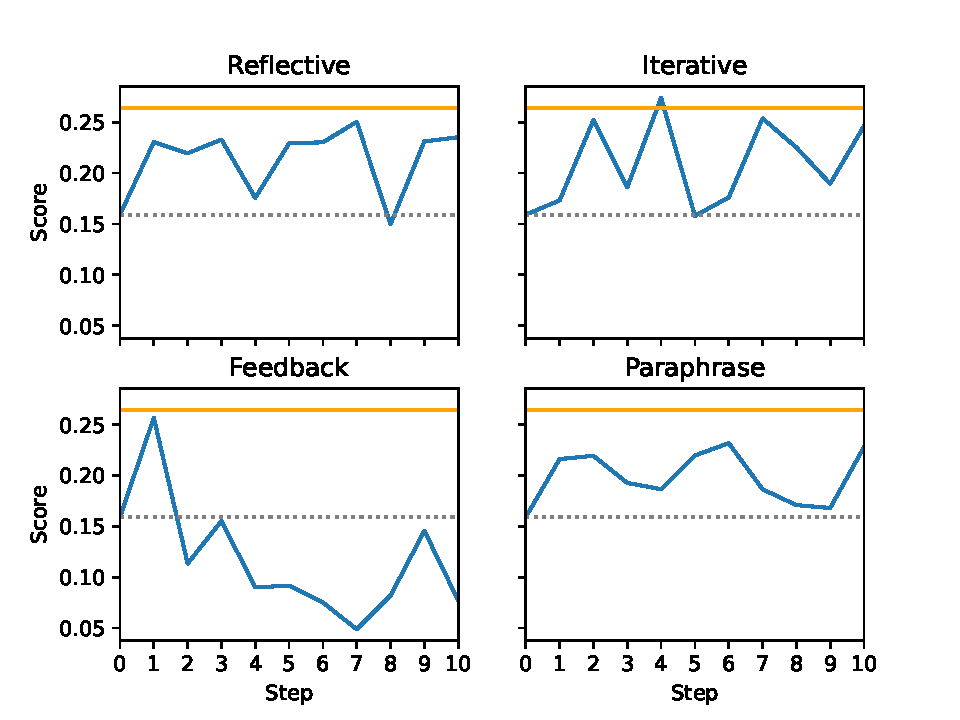
\includegraphics[width=\linewidth]{codecontests.pdf}
    \caption{Performance on CodeContests dataset}
\end{figure}
\begin{table}[htbp]
    \centering
    \captionsetup{font=small}
    \caption{Results for connections}  
    \label{tab:resconnections}
    \renewcommand{\arraystretch}{1.4} % row spacing

    \begin{tabular}{|c||c|c|c|c|}
    \hline
    \rowcolor{ctulightblue}
    \textsc{Step} &
    \cellcolor{ctulightblue}\textsc{Reflective} &
    \cellcolor{ctulightblue}\textsc{Iterative} &
    \cellcolor{ctulightblue}\textsc{Feedback} &
    \cellcolor{ctulightblue}\textsc{Paraphrase} \\
    \hline

    \rowcolor{ctuorange!15}
    Baseline & \textbf{0.33} & \textbf{0.33} & \textbf{0.33} & 0.33 \\ \hline
Initial & 0.20 & 0.20 & 0.20 & 0.20 \\ \hline
$1$ & \maxmean{0.29}{0.15} & \maxmean{0.27}{0.16} & \maxmean{0.20}{0.15} & \maxmean{0.31}{0.21} \\ \hline
$2$ & \maxmean{0.20}{0.13} & \maxmean{0.29}{0.18} & \maxmean{0.24}{0.14} & \maxmean{0.32}{0.20} \\ \hline
$3$ & \maxmean{0.20}{0.14} & \maxmean{0.27}{0.17} & \maxmean{0.19}{0.14} & \maxmean{0.29}{0.21} \\ \hline
$4$ & \maxmean{0.18}{0.04} & \maxmean{0.26}{0.17} & \maxmean{0.09}{0.06} & \maxmean{0.28}{0.19} \\ \hline
$5$ & \maxmean{0.16}{0.08} & \maxmean{0.27}{0.18} & \maxmean{0.14}{0.09} & \maxmean{0.31}{0.20} \\ \hline
$6$ & \maxmean{0.17}{0.09} & \maxmean{0.27}{0.19} & \maxmean{0.13}{0.08} & \maxmean{0.32}{0.21} \\ \hline
$7$ & \maxmean{0.16}{0.08} & \maxmean{0.29}{0.19} & \maxmean{0.10}{0.04} & \maxmean{0.30}{0.19} \\ \hline
$8$ & \maxmean{0.16}{0.08} & \maxmean{0.28}{0.19} & \maxmean{0.07}{0.04} & \maxmean{0.33}{0.23} \\ \hline
$9$ & \maxmean{0.16}{0.07} & \maxmean{0.27}{0.20} & \maxmean{0.05}{0.03} & \maxmean{0.28}{0.22} \\ \hline
$10$ & \maxmean{0.16}{0.07} & \maxmean{0.26}{0.16} & \maxmean{0.07}{0.03} & \maxmean{\underline{\textbf{0.35}}}{0.25} \\ \hline


    \end{tabular}
\end{table}

\begin{figure}
    \label{fig:connections}
    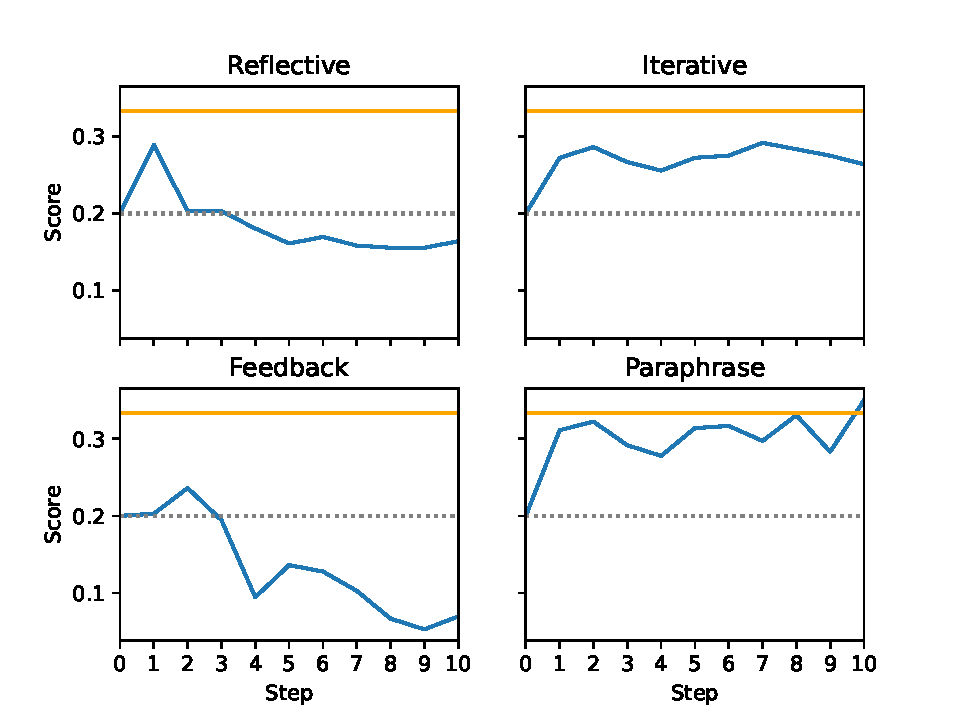
\includegraphics[width=\linewidth]{connections.pdf}
    \caption{Performance on connections dataset}
\end{figure}

\begin{table}[htbp]
    \centering
    \captionsetup{font=small}
    \caption{Results for sequences}  
    \label{tab:ressequences}
    \renewcommand{\arraystretch}{1.4} % row spacing

    \begin{tabular}{|c||c|c|c|c|}
    \hline
    \rowcolor{ctulightblue}
    \textsc{Step} &
    \cellcolor{ctulightblue}\textsc{Reflective} &
    \cellcolor{ctulightblue}\textsc{Iterative} &
    \cellcolor{ctulightblue}\textsc{Feedback} &
    \cellcolor{ctulightblue}\textsc{Paraphrase} \\
    \hline

    \rowcolor{ctuorange!15}
    Baseline & \textbf{0.70} & 0.70 & \textbf{0.70} & 0.70 \\ \hline
Initial & 0.40 & 0.40 & 0.40 & 0.40 \\ \hline
$1$ & \maxmean{0.47}{0.23} & \maxmean{0.63}{0.36} & \maxmean{0.43}{0.29} & \maxmean{0.73}{0.38} \\ \hline
$2$ & \maxmean{0.53}{0.39} & \maxmean{0.53}{0.32} & \maxmean{0.47}{0.32} & \maxmean{0.60}{0.33} \\ \hline
$3$ & \maxmean{0.27}{0.15} & \maxmean{0.67}{0.43} & \maxmean{0.47}{0.33} & \maxmean{0.63}{0.37} \\ \hline
$4$ & \maxmean{0.47}{0.21} & \maxmean{0.63}{0.42} & \maxmean{0.47}{0.32} & \maxmean{0.60}{0.42} \\ \hline
$5$ & \maxmean{0.57}{0.33} & \maxmean{0.63}{0.40} & \maxmean{0.40}{0.28} & \maxmean{0.60}{0.38} \\ \hline
$6$ & \maxmean{0.53}{0.35} & \maxmean{0.57}{0.34} & \maxmean{0.27}{0.19} & \maxmean{\underline{\textbf{0.80}}}{0.45} \\ \hline
$7$ & \maxmean{0.57}{0.44} & \maxmean{0.60}{0.31} & \maxmean{0.37}{0.23} & \maxmean{0.73}{0.37} \\ \hline
$8$ & \maxmean{0.63}{0.46} & \maxmean{0.70}{0.50} & \maxmean{0.37}{0.25} & \maxmean{0.57}{0.29} \\ \hline
$9$ & \maxmean{0.50}{0.40} & \maxmean{\underline{\textbf{0.80}}}{0.37} & \maxmean{0.43}{0.27} & \maxmean{0.63}{0.44} \\ \hline
$10$ & \maxmean{0.57}{0.41} & \maxmean{0.57}{0.39} & \maxmean{0.33}{0.21} & \maxmean{0.60}{0.35} \\ \hline


    \end{tabular}
\end{table}

\begin{figure}
    \label{fig:sequences}
    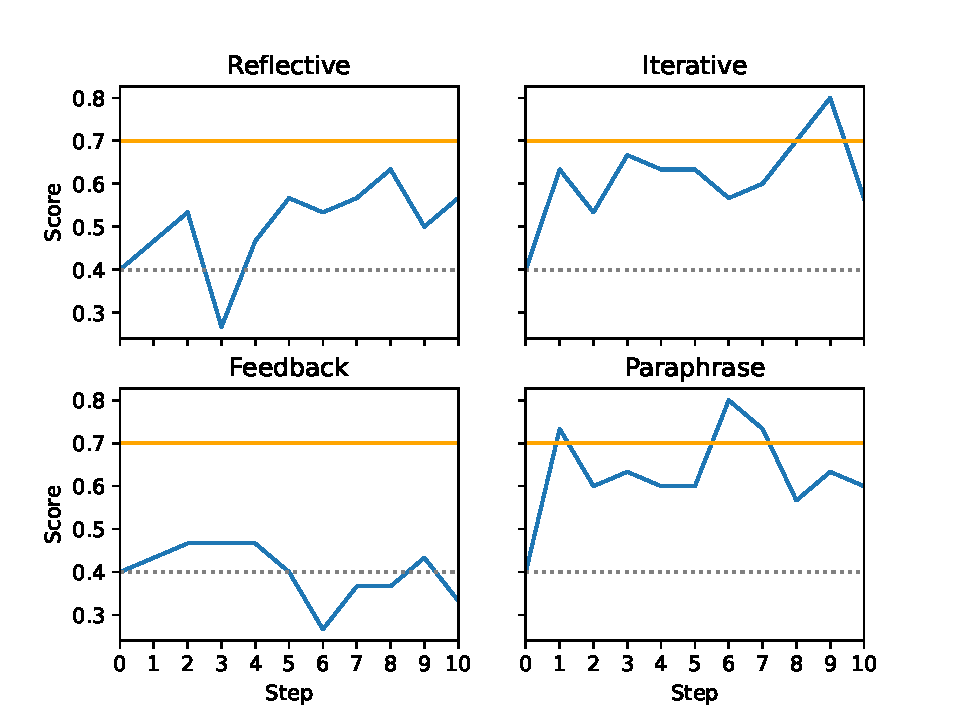
\includegraphics[width=\linewidth]{sequences.pdf}
    \caption{Performance on sequences dataset}
\end{figure}


\begin{figure}
    \label{fig:relative}
    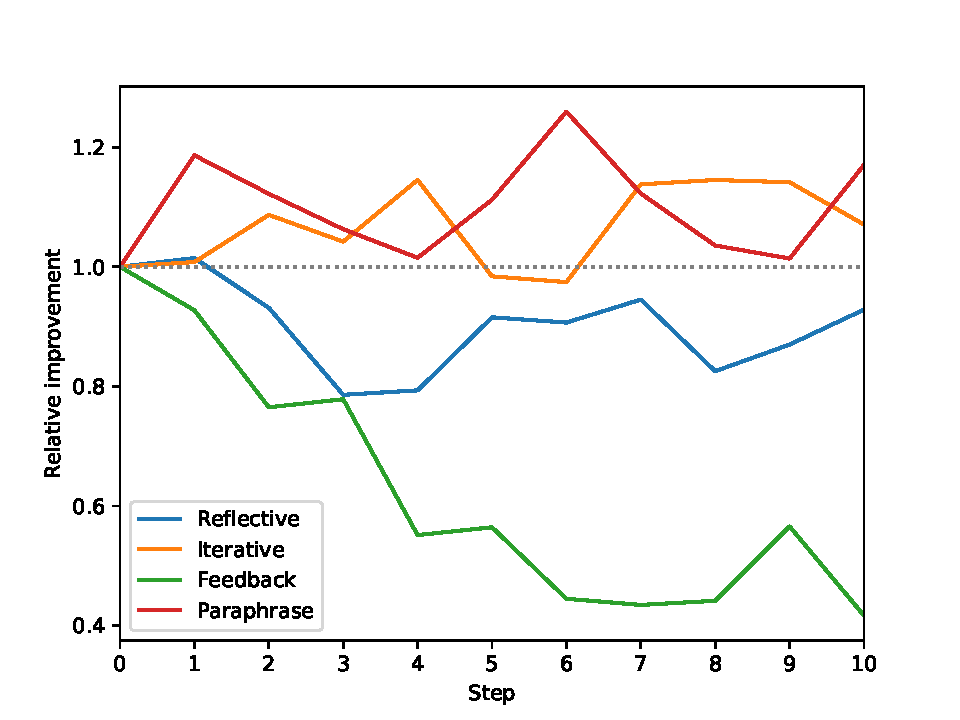
\includegraphics[width=\linewidth]{relative.pdf}
    \caption{Relative performance}
\end{figure}

\begin{figure}
    \label{fig:usage}
    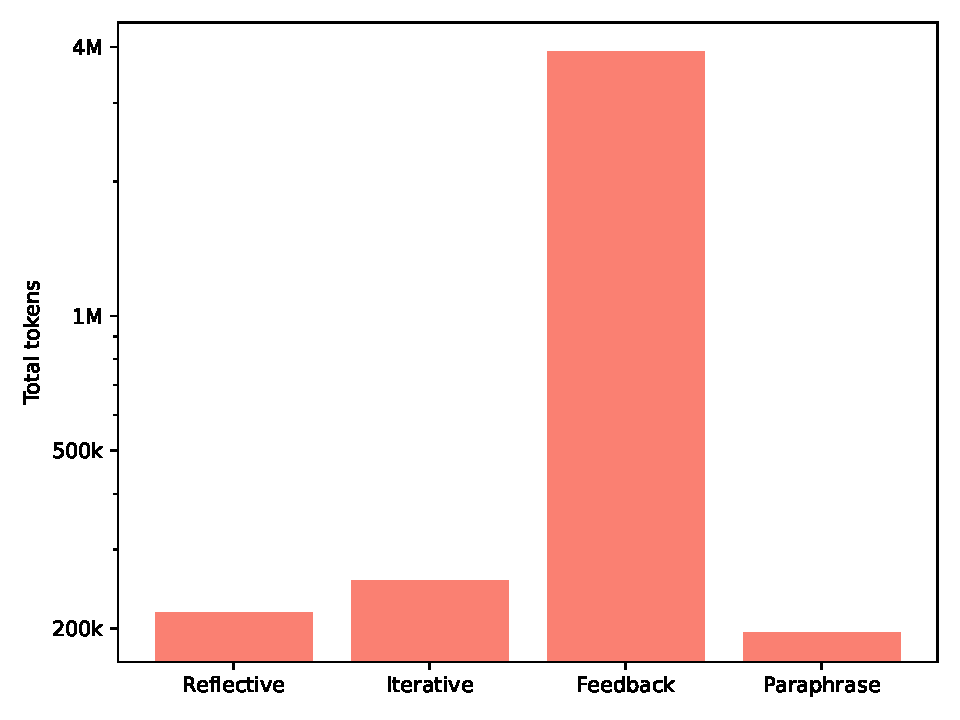
\includegraphics[width=\linewidth]{usage.pdf}
    \caption{Token optimization cost per operator}
\end{figure}

\newpage

\section{Self-Supervised Optimization for Open-Ended Tasks}
To showcase the applicability of our method on tasks without available gold labels, we conduct two experiments
on creative applications. The only designed operator applicable in self-supervised contexts is the \texttt{Feedback} 
operator which performs direct output and prompt comparisons.

\subsection{Limericks}
Limerick is a short humorous poem. We design a simple task, where the LLM has to write an alliterative limerick about an animal. 
All words should start with the starting letter of the animal given, for example:

\begin{promptbox}[label={box:limerick}]{Limerick task example}
    \textbf{Input}:
    \hlbox{ctuorange}{snake}
    \textbf{Output}:
    \hlbox{ctublue}{silly snakes swiftly slide,\\sneaky, slippery, side-to-side,\\slurping soda,\\singing sonata,\\simply sparkling, super-sized!}
\end{promptbox}

We provide three such examples without further context and observe the quality of the results. These examples are used to construct the initial population through
the \texttt{Lamarckian} operator.
We run the optimizer with population size $S=4$, iteration count $I=3$, batch size $B=1$ and pruning factor $f_{\text{prune}} = 0.5$.
The LLM of choice is again the \texttt{Google Gemma 3 27B} with $\tau = 0.75$ for $\mathcal{M}_{\text{optim}}$ and $\tau = 0.0$ for $\mathcal{M}_{\text{solve}}$

We present the best results from the initial population (generation $0$) and the last generation ($3$), as ranked by $\mathcal{M}_{\text{optim}}$.
The initial prompts already produce satisfactory results, with the winning result making sense and having only one error in alliteration.
However during the optimization, it seems that the comparison function started favoring longer results, consistent with findings of Ye et al.\cite{ye2024justiceprejudicequantifyingbiases}.
This problem originated in the first optimization step, where the \texttt{Feedback} operator created a prompt that instructed to "provide 3 different poem options".
Comparisons show that multiple options are preferred by the comparison function as they "showcase more variety and exploration of the theme".

\begin{promptbox}[label={box:limerickresult}]{Limerick optimization result}
\textbf{Initial}:
    \hlbox{ctulightblue}{
        daring dogs delightfully dash,\\
        dreaming deeply, a dazzling flash,\\
        digging daily,\\
        dancing daintily,\\
        devoted dreamers, a delightful dash!
    }
\textbf{Step 3}:
    \hlbox{ctulightblue}{
        daring dogs delightedly dash, \\
        dancing daily, a delightful flash, \\
        dreaming deeply, \\ 
        digging deftly, \\ 
        delicious dreams in a doggy splash. \\
\\
        dazzling dogs dreamily doze, \\ 
        delivering devotion, as everyone knows,\\ 
        dancing daily, \\
        delighting dually, \\
        deliciously drifting where the dandelion grows. \\
\\ 
        dynamic dogs diligently dive,\\ 
        discovering delights, truly alive,\\ 
        dreaming deeply,\\
        dancing steeply,\\
        daringly doing, to thrive and strive.
    }
\end{promptbox}

We conclude that our method failed to improve poem-generating prompts in this experiment, probably due to the 
ambiguous task definition, small population and batch sizes. Performance could be improved by designing 
a more specific operator set for creative tasks, as opposed our general-purpose operator set.

\subsection{Images}
We employ OpenAI's \texttt{Dall-E 3}\cite{BetkerImprovingIG} to demonstrate that our method can create prompts even for diffusion text-to-image models.
Learning from the failure from the previous experiment, we specialize the operator set for the task of image generation.
Utilizing the vision capabilities of \texttt{Google Gemma 3 27B}, the \texttt{Feedback} operator is modified to allow direct image comparisons. 

We choose the same hyperparameters as in the Limerick experiment. For the optimizer LLM, the vision-enabled \texttt{Google Gemma 3 27B} is used with $\tau = 0.75$ and 
$\mathcal{M}_{\text{solve}}$ is a diffusion text-to-image model \texttt{Dall-E 3} with image size $1024\times1024$ and default settings.

We select two triples of emotionally expressive adjectives and frame the optimization as a search for a prompt that creates an image best fitting this description. 
The first triple is "wistful", "hopeful", "lonely" and the second is "graceful", "furious", "vulnerable". In figures \ref{fig:wistful} and \ref{fig:graceful} the reader can find
highest win rate images from each optimization step.


\begin{figure}[htbp]
    \centering

    \begin{subfigure}{0.24\linewidth}
        \includegraphics[width=\linewidth]{image-gen0-id725f8.jpg}
        \caption{Initial}
    \end{subfigure}
    \hfill
    \begin{subfigure}{0.24\linewidth}
        \includegraphics[width=\linewidth]{image-gen1-id534fc.jpg}
        \caption{Step 1}
    \end{subfigure}
    \hfill
    \begin{subfigure}{0.24\linewidth}
        \includegraphics[width=\linewidth]{image-gen2-id62971.jpg}
        \caption{Step 2}
    \end{subfigure}
    \hfill
    \begin{subfigure}{0.24\linewidth}
        \includegraphics[width=\linewidth]{image-gen3-id4cf7b.jpg}
        \caption{Step 3}
    \end{subfigure}

    \caption{Best images from each optimization step for the words "wistful", "hopeful" and "lonely".}
    \label{fig:wistful}
\end{figure}

\begin{figure}[htbp]
    \centering

    \begin{subfigure}{0.24\linewidth}
        \includegraphics[width=\linewidth]{image-gen0-id1de72.jpg}
        \caption{Initial}
    \end{subfigure}
    \hfill
    \begin{subfigure}{0.24\linewidth}
        \includegraphics[width=\linewidth]{image-gen1-id4edb5.jpg}
        \caption{Step 1}
    \end{subfigure}
    \hfill
    \begin{subfigure}{0.24\linewidth}
        \includegraphics[width=\linewidth]{image-gen2-id6a3db.jpg}
        \caption{Step 2}
    \end{subfigure}
    \hfill
    \begin{subfigure}{0.24\linewidth}
        \includegraphics[width=\linewidth]{image-gen3-id622c1.jpg}
        \caption{Step 3}
    \end{subfigure}

    \caption{Best images from each optimization step for the words "graceful", "furious" and "vulnerable".}
    \label{fig:graceful}
\end{figure}

All generated images reflect the target description and, as artistic taste is subjective, we will leave it to the reader 
to decide if the optimized prompts produce better images. We observe, that in \ref{fig:wistful}, the image seems to get more personal as it zooms in on the subject.
The winning images are all in a very similar style. This is in contrast to \ref{fig:graceful}, where the focus seems to have shifted to 
photorealistic images in the first optimization step.

Note that in this case, the optimization is framed in a different manner from previous experiments.
We are conducting "run-time" optimization for a particular task instance unlike previous "compile-time" experiments, where we optimized for a whole task class.
